\chapter{Fault detection in Utility Scale Photovoltaic Plants} \label{chap:chap2}


\section{Utility-Scale Photovoltaic System's Architecture}

Utility-scale photovoltaic (PV) power plants are large-scale PV systems that are connected to the electrical grid and have installed capacities ranging from kilowatts peak (kWp) to megawatts peak (MWp). These systems typically consist of many PV panels interconnected through power electronics to aggregate and inject active power into the grid. The number and type of components in a PV power plant depend on the plant's scale and topology, with different configurations possible for large-scale applications, including central inverters, string inverters, and multi-string inverters \cite{lspv}. Understanding the architecture and components of PV power plants is vital for designing, operating, and maintaining these systems, as it helps optimize their performance and reliability.

\begin{figure}[h]
    \centering
    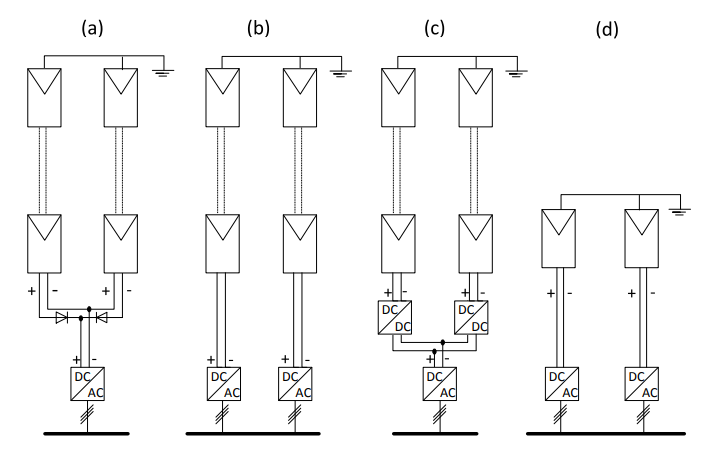
\includegraphics[width=12cm]{figures/topologies.png}
    \caption{PV inverter topologies:  (a) Central, (b) String, (c) Multi-string,
    (d) Module integrated \cite{lspv}.}
    \label{topologies}
\end{figure}

In figure \ref{topologies}, the fourth configuration presented (d) will not be considered for utility-scale plants due to its expensive nature. After DC/AC conversion, another voltage conversion step usually establishes the grid connection: an AC/AC transformer.

For completeness, the physical installation of PV modules can include solar tracking apparatuses, such as single and dual-axis trackers, which add to system complexity and change production behavior. Nonetheless, and turning the focus back toward the electrical components, the main ones are the following:

\begin{itemize}
    \item Solar photovoltaic panels.
    \item Electric cabling.
    \item Inverter(s) (mostly with Max Power Point Trackers).
    \item AC Transformer(s).
    \item Protection components (circuit breakers, fuses, surge protectors,
    etc.)
\end{itemize}

Most of these components have intrinsic variables, such as voltage and current values, that can help determine their operation states. Given that the utility grids (and the associated electricity market) integrate large-scale PV assets, some of the before-mentioned components require constant monitoring and control, achieved with adequate embedded systems and sensor infrastructure \cite{AIPV}. Thanks to the continuous advancements in communication technologies, namely in IoT (Internet Of Things), data acquisition is becoming faster, more reliable, and more precise. Not only is this fundamental for real-time asset assessment, but it also allows better training of prediction algorithms. However, on the industrial scale (in the order of MWp production), having sensors embedded in every PV module comes with a high economical cost, and inverters are the components that usually possess monitoring capabilities. Since monitoring utility-scale PV assets rely on the investment and technologies employed for this purpose,  engineers must consider data availability when developing data-driven algorithms, such as forecasting and fault detection.

\section{Types of faults}

Several types of faults can occur in utility-scale photovoltaic (PV) power plants, which can negatively impact the performance and reliability of the system, possibly causing safety hazards \cite{Alam2015}. Some are challenging to detect and protect the electrical installation against, thus requiring sophisticated detection algorithms \cite{Pillai2018}. According to \cite{Pillai2018}, these faults can fit into three categories: electrical, mechanical, and environmental. Electrical faults include short circuits, open circuits, and inverter failure, affecting the PV panels' power output and the system's overall efficiency. Mechanical faults include broken panels, damaged cables, and defective inverters, which can lead to system downtime and reduced performance. Environmental faults include extreme weather events, such as hail or strong winds, which can damage the PV panels and other components \cite{faults}. Figure \ref{fig: faults} illustrates a more extensive summary of fault types.

\begin{figure}[h]
    \centering
    \includegraphics[width=16cm, trim={2cm 2.1cm 2cm 12cm},
    clip]{figures/chapter2/types\_of\_faults.pdf} \caption{"Classification of
    faults in PV Systems", from \ref{Pillai2018}.}
    \label{fig:faults}
\end{figure}

Throughout the literature \cite{Braun2011}, some of the most studied faults in the context of fault detection are:

\begin{itemize}
    \item Shading: partial coverage, temporary or not, of a PV array or module. It might result in a Hot Spot fault.
    \item Soiling: dirt accumulation, blocking sunlight from reaching PV Cells. It might also result in a Hot Spot fault.
    \item Short circuit: either line-line or line-ground.
    \item Open circuit: connection breakage between modules.
    \item DC arc fault: electricity plasma arc formed on broken connections.
\end{itemize}

According to a 2017 survey conducted on five utility-scale PV plants in Italy, the authors observed failure rates from
<1\% to 3\% in the majority of plants, and 81.8\% on the worst scenario \cite{Grimaccia2017}. The high failure rate of
the latter had a demonstrated cause that originated from manufacturing mistakes: snail trails. Besides this phenomenon,
hot spot faults and bypass diode faults/disconnections were among the most common.

\begin{figure}[h]
    \centering
    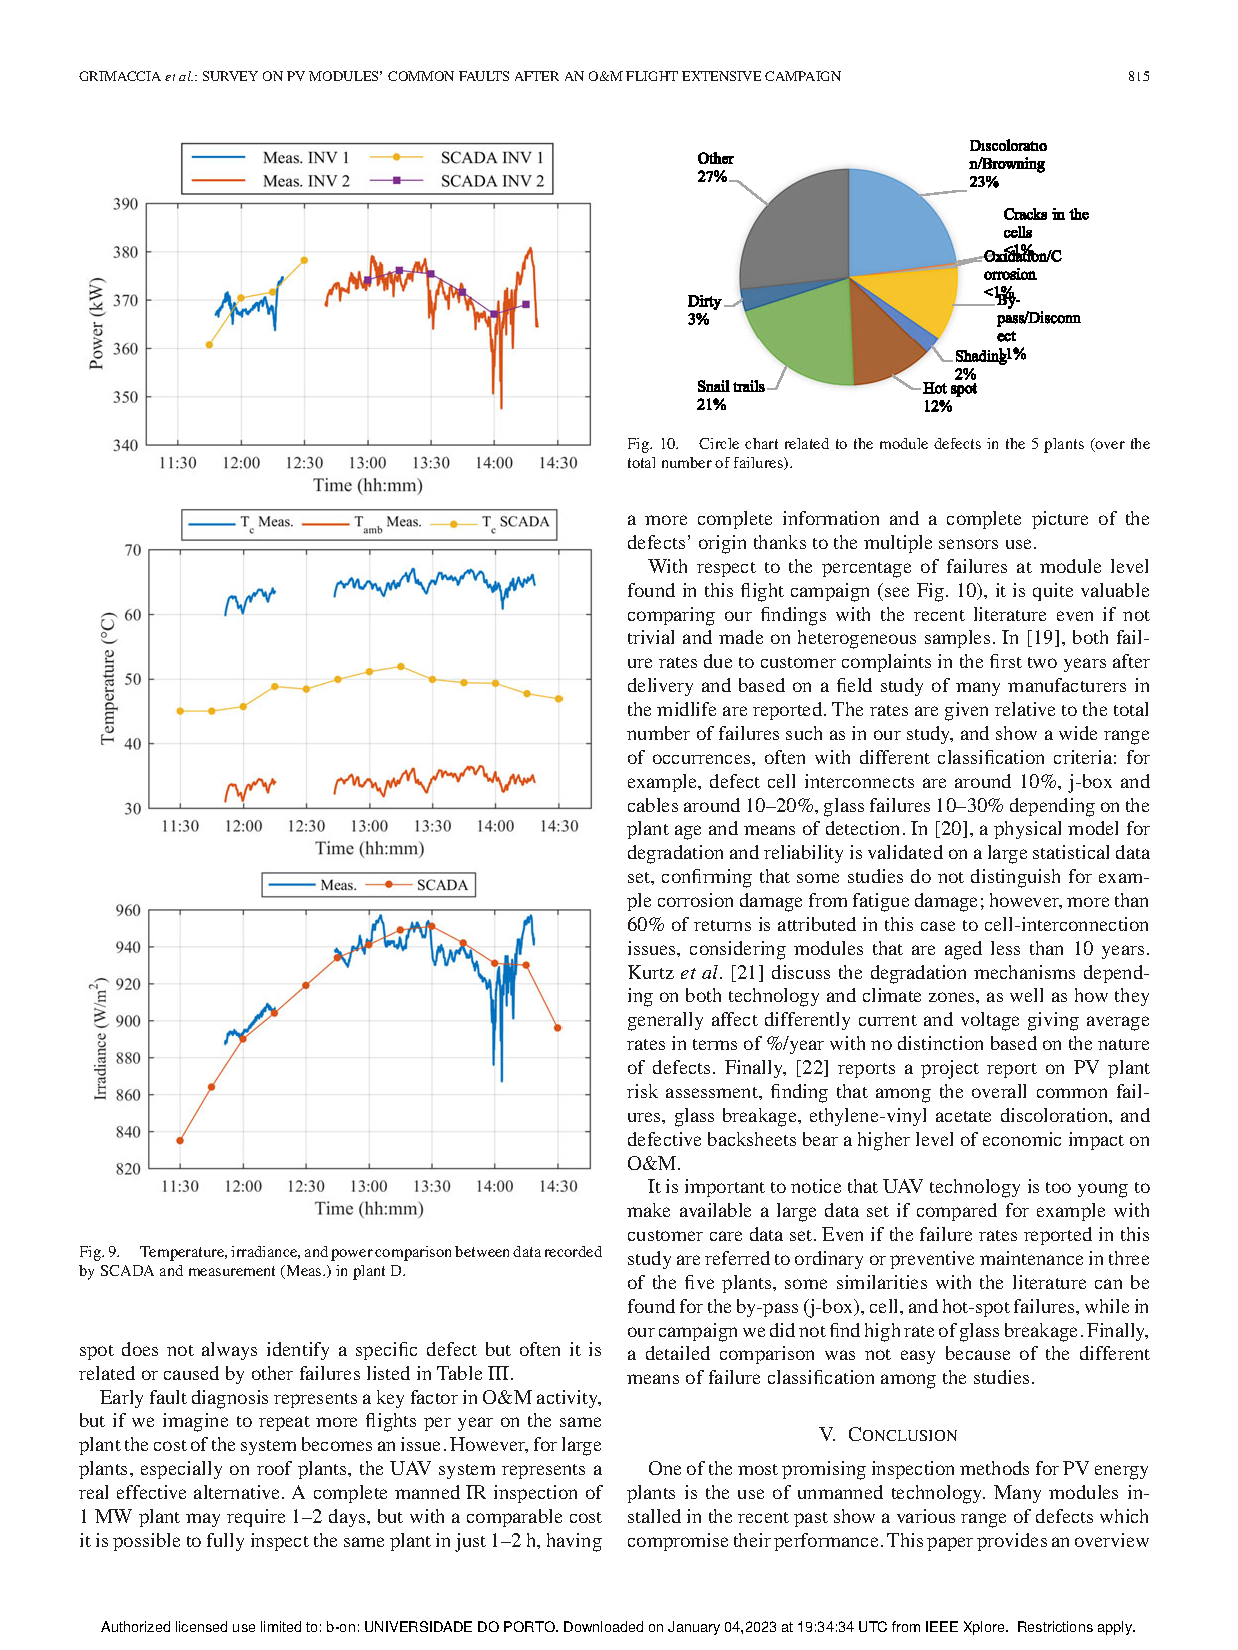
\includegraphics[width=10cm, trim={11cm 20.6cm 2.4cm 2cm},
    clip]{figures/chapter2/chartfailsurvey.pdf} \caption{"Circle chart related to the module defects in the 5 plants
    (over the total number of failures)", from \ref{Grimaccia2017}.}
    \label{fig:faultchart}
\end{figure}

Having the distribution of fault types from real-life scenarios is quite helpful for formulating fault detection algorithms. It allows for better generation/selection of training data and decision of classes. In figure \ref{fig:faultchart}, it is possible to observe the failure type distribution for 24.254 inspected modules. Soiling, shading, and mechanically related failures were not as prominent, with only a group share of around 6\%. It is relevant to note that discoloration represents almost a quarter of all faults.

Although the study had a limited geographic scope, with only a few power plants diagnosed, it allows for a more realistic view of the common scenarios encountered in typical operational ground-mounted utility-scale PV power plants.

Due to the difficulty of classifying some of these faults, given their similarity on the consequent effect in the system, it will be seen in further sections that most fault detection algorithms only endeavor to classify between two to five types of reviewed faults.

\section{Modeling photovoltaic's physical/electrical behavior}

Photovoltaic cells are the fundamental components of photovoltaic panels. They are made from semiconductor materials, such as silicon,  and absorb photons that generate an electric current. Their electrical behavior is characterizable using the current-voltage (I-V) equation. This equation, which represents a fundamental relationship governing the operation of PV cells, can be used to predict their performance under various operating conditions, such as solar irradiance and temperature.

For state estimation, it is crucial to accurately model PV modules' performance from the DC side of power converters. This information is vital for designing and optimizing PV power systems, as it enables predicting PV module performance under different conditions, as mentioned before. Accurate PV module models are also essential for state estimation and fault detection, as they provide critical information about the health and performance of PV modules, allowing for early identification of potential issues. In addition, they can be used to optimize the control and operation of PV power systems, which can improve the overall efficiency and reliability of the system \cite{Braun2011}.

Physical and empirical models broadly categorize the several state-of-the-art methods for modeling photovoltaic modules \cite{Braun2011}. Physical models lie on the fundamental physical principles governing PV modules' operation. They typically require detailed knowledge of the PV module's electrical and optical properties, such as its current-voltage (I-V) characteristics, spectral response, and temperature dependence. These models can accurately predict the PV module's performance under a wide range of operating conditions, but they may be complex and computationally intensive to implement \cite{Kumar2019}. On the other hand, empirical models are based on experimental data and are typically more straightforward to implement. However, they may not be as accurate as physical models, especially under conditions that differ significantly from those used to generate the experimental data (usually STC) \cite{Braun2011}. Some examples of state-of-the-art physical models for PV modules include the single-diode model (also known as the five-parameter model), and the two-diode model \cite{Godina2017}. In contrast, one of the most used state-of-the-art empirical models is the Sandia model \cite{Braun2011}. The choice of modeling method will depend on the specific application and the required level of accuracy and complexity; in some cases, there can be a combination of physical and empirical models.

Suppose the need arises to model PV modules in this work. In that case, it is critical to select a simple methodology so that the module's datasheet characteristics are sufficient to model the PV arrays accurately. In the case of utility-scale PV systems, detailed knowledge of the module's electrical and optical properties of empirical data may be limited, and building a model is only possible by using datasheet data. A complex model that requires more detailed information may not be feasible in such cases, and a simpler model that relies on fewer input parameters is more appropriate. The single-diode model seems appropriate for this use case, given the excellent trade-off between complexity and accuracy.

\subsection{The five-parameter model}

The single-diode model representation of the photovoltaic module is presented in figure \ref{}. The I-V curve can be obtained by numerically solving the following equation:

\begin{equation}
I = I_{L} - I_{0} \times (e^{\frac{V + I \times R_{s}}{n \times V_T}} - 1)
\end{equation}

where $I_{L}$ is the light-generated current, $I_{0}$ is the reverse saturation current, $R_{s}$ is the series resistance, $n$ is the ideality factor, and $V_{T}$ is the thermal voltage. These parameters are determined by fitting the model to experimental data or using data from the PV module's datasheet. The single-diode model can predict the PV module's performance under a wide range of operating conditions while maintaining reasonable accuracy. However, remembering that the single-diode model is a simplified representation of the PV module, it will have poor accuracy under certain conditions compared to the more representative two-diode model \cite{Godina2017}.

% insert image here

\section{Literature on Fault detection for Photovoltaic Systems}

The parent field of fault detection is anomaly detection (also known as outlier detection), a highly studied subject in the scope of statistics \cite{Prasad2009}, applied in many scientific areas. The tools dedicated to fault detection and state estimation mostly come from mathematical/statistical methodologies, machine learning, and deep learning applications \cite{AIPV}. Parting from the three general problem-solving principles mentioned before, machine learning and deep learning are the most popular and successful ones for recent applications that ought to solve a plethora of complex problems. Such potential has led to an interest in their usage for implementing fault detection algorithms.

\subsection{Statistical and Signal Processing Algorithms}

Statistical methodologies look into historical data to find the characteristics of how samples relate to the population (interpolation). These methodologies yield good results in case studies of PV farms that have been logging data for a considerable time, suffering in the cases that do not. Therefore, they are limited in that it is required to have curated data sets of historical significance for relevant features of the studied systems.

% write about signal processing

For the field of fault detection in PV systems, the literature on statistical and signal processing algorithms is mostly quite dated (\cite{Buddha2012}, \cite{Zhao2014}, \cite{Vergura2008}), given that more recent machine learning methods became increasingly interesting for this matter. Nonetheless, anomaly (or outlier) detection statistical algorithms can be used for fault detection in PV systems by identifying unusual patterns or deviations from normal behavior in the data collected from the PV system. For this, we might employ distance-based methods, such as Euclidean, Mahalanobis, and MCD-based distances \cite{Braun2011}. Although simple, distance-based techniques only might work for detecting outliers in the context of PV systems if they are scale-invariant (due to the different magnitude in the system's state variables) and resilient to outlier contamination (only with MCD-based distance). In  \cite{Vergura2008}, the authors applied Analysis of Variance (ANOVA) and Kruskal-Wallis test for inverter failure detection, with the downside of only being able to identify outliers in a sub-array resolution, i.e., not for specific string or module failures.

% should graph signal processing be here too?

\subsection{Machine Learning Algorithms}

Machine learning came to solve some of the complications referred to in the two past subjects, as neural networks (or other learning structures) are easily capable of modeling complex, non-trivial, and nonlinear relations between data. Still, they are as good as the training data, with many structures requiring many representative learning examples to achieve good results. Their output can also be very obfuscated, meaning that many methods do not allow a direct interpretation of the relationship between inputs and outputs. This "black-box" characteristic, specifically of neural networks, is considered a disadvantage. Besides, extrapolating data remains a challenge when classically using these structures. Still, they have immense applications for PV systems, from MPP (Max Power Point) estimation to power forecasting, soiling, and fault prediction.

\subsection{Deep Learning Algorithms}

The field of deep learning branches off from machine learning, with the term "deep" referring to amplified machine learning structures that ought to understand data patterns through numerous intertwined neuron connections. A simple example of a deep learning model would be the design of an artificial neural network with multiple hidden layers (multidimensional), with the intuition that each of these "extra" layers achieves feature/pattern recognition in a cascade. They have been explored alongside machine learning techniques for PV fault detection, although the known disadvantage is a usually high computational cost and relatively tricky implementation.


While classical fault detection lies in the synchronous and direct evaluation of state estimation variables, fault prediction requires the input of time-series features. Although relatively simple, some classical time-series forecasting and analysis tools can be of great support to help design a fault prediction algorithm, such as Box-Jenkins methods and the Partial Auto-correlation function. Still, the majority of modern prediction tools comprise neural networks and variations. With this in mind, recent developments in the intelligent composition of learner structures spark some interest in the application to this field, such as the new deep learning technique named Cell Complex Neural Networks \cite{Hajij2020}. Further investigation of such modern practices will unroll throughout the development of this work.

